\begin{figure}[t]
\centering
\begin{subfigure}{.32915\linewidth}
\centering
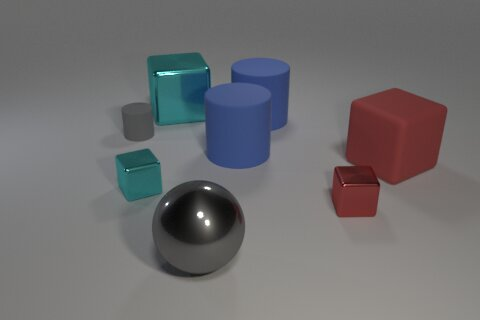
\includegraphics[width=\linewidth]{figures/clevr/input/0.jpg}\\
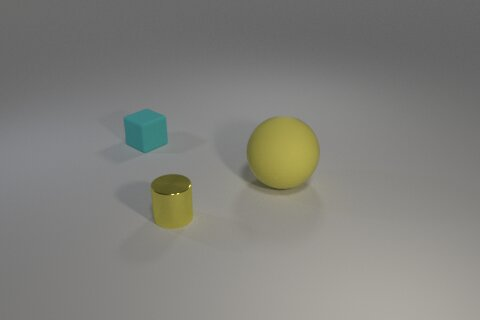
\includegraphics[width=\linewidth]{figures/clevr/input/1.jpg}
\caption{Input}
\end{subfigure}
\hfill
\begin{subfigure}{.32915\linewidth}
\centering
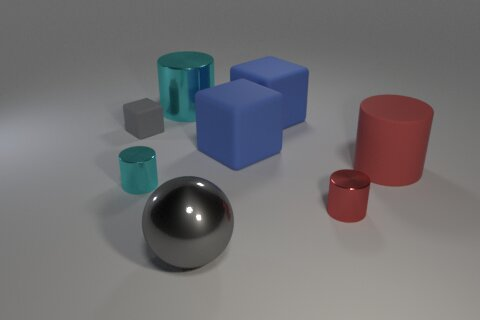
\includegraphics[width=\linewidth]{figures/clevr/ns-vqa/0.jpg}\\
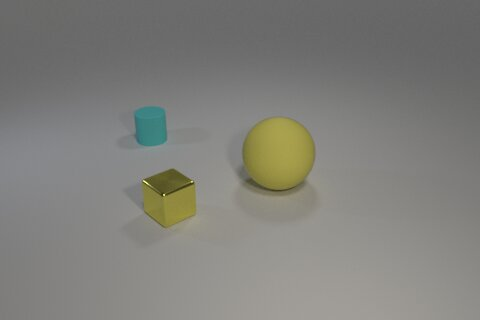
\includegraphics[width=\linewidth]{figures/clevr/ns-vqa/1.jpg}
\caption{NS-VQA}
\end{subfigure}
\hfill
\begin{subfigure}{.32915\linewidth}
\centering
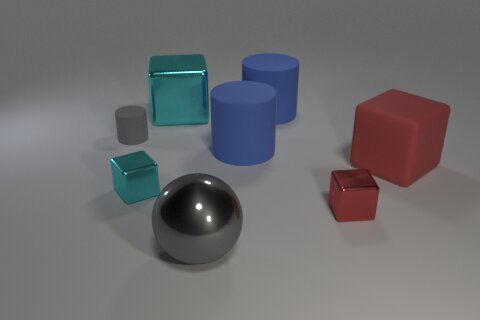
\includegraphics[width=\linewidth]{figures/clevr/output/0.jpg}\\
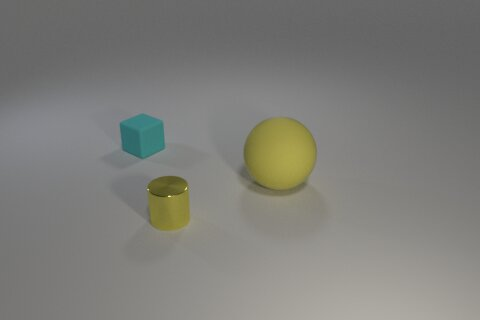
\includegraphics[width=\linewidth]{figures/clevr/output/1.jpg}
\caption{Ours}
\end{subfigure}
\caption{\textbf{OOD CLEVR-CoGenT Samples.} (\cref{ssec:clevr})
NS-VQA, with its modular design, fails to disentangle shape from color, while our framework is able to effectively generalize to OOD attribute combinations.
See \cref{fig:clevr_samples_additional} for additional samples.
}
\label{fig:clevr_samples}
\end{figure}